%%% Local Variables: 
%%% mode: latex
%%% TeX-master: t
%%% End: 

\chapter{支持向量机分类与后续处理}
 图像分割问题本质上是一个分类问题,图像中的所有像素都被分成两类或者更多类。每一类像素都有共有的特征,分类过程通过这些特征将每一类区分出来。传统的分类方法有监督方法和非监督方法,比如说支持向量机\cite{cortes1995support},K-means聚类方法\cite{macqueen1967some}和朴素贝叶斯分类器\cite{rish2001empirical}等。本文采用支持向量机来对角毛藻显微图像中的所有像素进行分类,待处理图像中的像素被分为两类:目标部分(角毛藻)和背景部分。由于经过分类后的图像并没有完全把目标分离出来,因此还需要通过后续处理来生成最终的分割结果。

\section{支持向量机}
支持向量机(Support Vector Machine,SVM)理论,是Corinna Cortes和Vapnik\cite{cortes1995support}等于1995年首先提出的,因为它在解决非线性、小样本及高维模式识别中表现出许多特有的优势,并且能推广应用到其他机器学习问题中,所以一直被认为是效果最好的可用的分类算法之一。在机器学习领域中,受到越来越多的广泛关注。

传统的学习方法一般是通过最小化经验风险(Empirical Risk Minimization,ERM)来实现的。但是当只有有限个训练样本时,经验风险最小化原则一般是不合理的,并且ERM算法在实际应用中会遇到不适定等问题。

支持向量机是通过寻求结构化风险最小来提高学习机的泛化能力,最小化经验风险和置信范围以达到在样本量较少情况下仍能获得较好统计规律的目的。其基本思想是:当样本集是线性时,两类样本通过寻找最优分类超平面来区分;当样本集是非线性时,需要将低维空间映射到高维空间来寻找最优分类超平面。支持向量机通过使用具有某些特殊性质的核函数将特征空间中的内积运算转换为在低位空间里的非线性运算,避免了高维空间的计算问题。
    
\subsection{实际风险、经验风险与结构风险}
\subsubsection{实际风险}
假设学习机器广义参数为$\omega$,那么对于输入量和输出量分别为$x$和$f(x,\omega)$的学习机器,其预测的实际风险为:
\begin{equation}
R(\alpha)=\int L(y,f(x,\omega))dF(x,y)
\end{equation}
$F(x,y)$为变量$x$和$y$之间的联合分布,$L(y,f(x,\omega))$则为损失函数,即预测输出$f(x,\omega)$对实际输出$y$预测产生的损失。

\subsubsection{经验风险}
在实际应用中,联合分布$F(x,y)$是不可能得到的,经验风险最小化原则一般会通过样本来对经验风险定义:
\begin{equation}
R_{emp}(\omega)=\frac{1}{n}\sum_{i=1}^{n}L(y_{i}.f(x_{i},\omega))
\end{equation}

优化机器学习就是要找到一个最优广义参数$\alpha$并最小化$R(\alpha)$,最小化经验风险实质上就是使经验风险逐渐趋近于实际风险的过程。

此外由于经验风险是基于大数定律得到的,$R_{emp}$只有样本趋于无穷时才能在概率意义上趋于$R(\alpha)$。因此在样本数有限的情况下是否能取得良好的结果仍然缺乏理论支持。

\subsubsection{结构风险}
对于所有预测函数来说,$R(\alpha)$与$R_{emp}$间以大于等于$1-\eta$的概率满足以下关系:
\begin{equation}\label{gongshi}
R(\alpha)\le R_{emp}(\omega)+\sqrt{\frac{(h(\ln(\frac{2n}{h})+1)-\ln(\frac{\eta}{4})}{n}}
\end{equation}
其中,$n$表示样本数,$h$表示函数集的VC维(Vapnik-Chervonenkis Dimension),由式\ref{gongshi}可知,置信范围和经验风险两部分共同组成了实际风险。在实际机器学习过程中,最小化经验风险同时尽最大可能减少置信范围,并且按照VC维的大小,综合衡量$R_{emp}$和函数子集间的置信范围来获取$R(\alpha)$的最小值的思想就是结构风险最小化(Structural Risk Minimization),即SRM准则。

\subsection{线性情况与非线性情况} 
\subsubsection{线性情况} 

首先考虑一个两类的分类问题,数据点$x$是一个$n$维向量,类别用$y$表示,取值可以是$1$或$-1$。线性分类器就是要从$n$维的数据空间中找出一个超平面来将整个数据空间分为两类,其方程可以表示为:
\begin{equation}
w^{T}x+b=0
\end{equation}
一个超平面在二维空间中就是一条直线,令分类函数$f(x)=w^{T}x+b$,当$f(x)=0$时,$x$是位于超平面上的点。对于所有满足$f(x)<0$的点,其对应的$y=-1$;而满足$f(x)>0$则对应$y=1$的数据点。$\vert f(x)\vert$越大分类越容易,当$\vert f(x)\vert=0$或$\vert f(x)\vert$值很小时,通常情况下很难处理。因为出现比较细微的变动(比如超平面转动了一个很小的角度时)很可能会导致分类结果的变化。直观几何意义上来说,越远离超平面的点越容易分类,而接近超平面的点往往很难分类。
\begin{figure}[ht!]
   \centering
  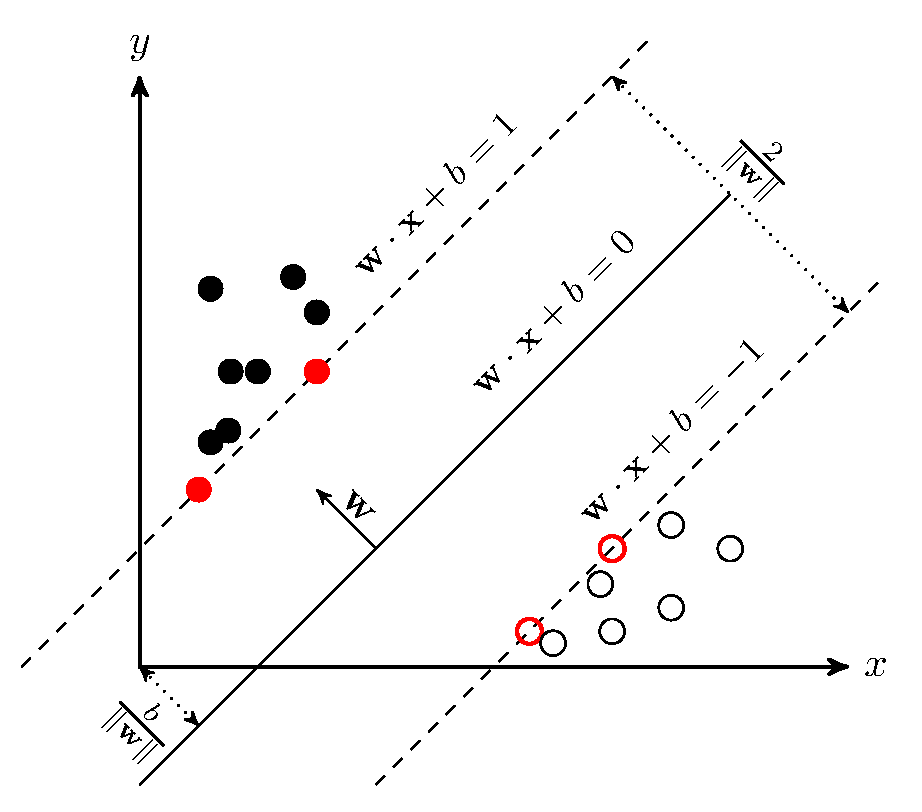
\includegraphics[width=0.9\linewidth]{svm.png}
  \caption{最优超平面}
    \label{}
 \end{figure}


假设一个数据点$x$投影到超平面上为$x_{0}$,$w$为垂直于超平面的矢量,则$x$到超平面的几何间隔为:
\begin{equation}
\hat{\gamma}=y\gamma=\frac{\hat{\gamma}}{\Vert{w}\Vert}
\end{equation}
其中$\hat{\gamma}$为函数间隔,且$\hat{\gamma}=y(w^{T}x+b)=yf(x)$,当对数据点进行分类时,集合间隔越大,分类置信就越高。因此为了使得分类的置信高,希望选择的超平面能够最大化几何间隔,定义目标函数为:
\begin{equation}
\max \hat{\gamma}
\end{equation}
当然还需要满足一些条件,根据间隔的定义,有:
\begin{equation}
y_{i}(w^{T}x+b)=\hat{\gamma_{i}}\ge\hat{\gamma},i=1,...,n
\end{equation}
为了优化和方便推导,令$\hat{\gamma}=1$,则上述目标函数变为:
\begin{equation}
\max\frac{1}{\Vert{w}\Vert},s.t.,y_{i}(w^{T}x+b)\ge1,i=1,...,n
\end{equation}
上述问题等价于:
\begin{equation}
\max\frac{1}{2}\Vert{w}\Vert^{2},s.t.,y_{i}(w^{T}x+b)\ge1,i=1,...,n
\end{equation}
使用拉格朗日优化法改造上式,即在满足$\sum_{i=1}^{n}y_{i}\alpha_{i}=0$
和$\alpha_{i}\ge0,i=1,...,n$的约束条件下,求解下式:
\begin{equation}
Q(\alpha)=\max \sum_{i=1}^{n}\alpha_{i}-\frac{1}{2}\sum_{i,j=1}^{n}\alpha_{i}\alpha_{i}y_{i}y_{j}(x_{i}\bullet x_{j})
\end{equation}
$\alpha_{i}$是每一个样本对应的拉格朗日乘子,上式有唯一解,只有当对应样本是支持向量时,$\alpha_{i}$不为零。则可以得到最优分类函数为:
\begin{equation}
g(x)=\textrm{sgn}\{(w\bullet x)+b\}=\textrm{sgn}\Big \{\sum_{i=1}^{n}\alpha_{i}^{*}y_{i}(x_{i}\bullet x)+b^{*}\Big \}
\end{equation}
只需要对支持向量求和并计算任意一对支持向量的中指或代入到任意一个支持向量都可以求出分类阈值$b^{*}$。

\subsubsection{非线性情况} 
当需要分类的训练集是非线性时,需要通过映射$\phi(\cdot)$将训练集映射到高维空间上。在高维空间上,训练集是线性可分的,决策函数可以通过采用线性情况的形式来构造最优分类超平面。支持向量机允许数据点在一定程度上偏离超平面。此时,约束条件变为:
\begin{equation}
y_{i}(w^{T}x+b)\ge 1-\xi_{i},i=1,...,n
\end{equation}
$\xi_{i}$是松弛变量,表示数据点$x_{i}$允许偏离的函数间隔值。此时的目标函数为:
\begin{equation}
\min\frac{1}{2}\Vert{w}\Vert^{2}+C\sum_{i=1}^{n}\xi_{i}
\end{equation}
\begin{equation}
s.t.,y_{i}(w^{T}x_{i}+b)\ge1-\xi_{i},i=1,...,n,\xi_{i}\ge0,i=1,...,n
\end{equation}
$C$为确定的常量,用以控制确保数据点偏差最小且能够找到间隔最大超平面的权重。$\xi$为待优化变量,目标函数为:
\begin{equation}
Q(\alpha)=\max \sum_{i=1}^{n}\alpha_{i}-\frac{1}{2}\sum_{i,j=1}^{n}\alpha_{i}\alpha_{i}y_{i}y_{j}K(x_{i},x_{j})
\end{equation}

\begin{equation}
s.t.,0\le\alpha_{i}\leC,i=1,...,n,\sum_{i=1}^{n}\alpha_{i}y{i}=0
\end{equation}
对应的分类函数变为:
\begin{equation}
g(x)=\textrm{sgn}\Big \{\sum_{i=1}^{n}\alpha_{i}^{*}y_{i}K(x_{i},x)+b^{*}\Big \}
\end{equation}

其中$K(x_{i},x_{j})=\phi(x_{i})\cdot\phi(x_{j})$为核函数。

\subsection{常见的核函数} 
当处于非线性情况时,需要将训练集映射到高维空间来寻找最优分类超平面。然而点积运算量会随着空间维数的增大而增大,这会产生“维数灾难”。支持向量机需要使用核函数来克服“维数灾难”,在选取核函数时需要满足Mercer条件,即:

\begin{equation}
\iint K(x_{i},x_{j})\phi(x_{i})\phi(x_{j})dx_{i}dx_{j}>0
\end{equation}
其中$\int\phi^{2}(x)dx<\infty$且$\phi(x)$不恒为零。
在实际情况下,通常用到以下三个核函数:
\begin{enumerate}
\item多项式核函数:
\begin{equation}
K(x_{i},x_{j})=[\gamma x_{i}\bullet x_{j}+r]^{d}
\end{equation}
\item径向基核函数:
\begin{equation}
K(x_{i},x_{j})=\exp\Big\{-\frac{\Vert x-x_{i}\Vert^{2}}{\sigma^{2}}\Big\}
\end{equation}
\item Sigmoid函数:
\begin{equation}
K(x_{i},x_{j})=\tanh[\gamma x_{i}^{T}\bullet x_{j}+r]
\end{equation}
\end{enumerate}

\section{实验结果}
本文使用支持向量机来对待处理图像中的像素进行分类,支持向量机的分类过程分为训练过程和预测过程。
\begin{enumerate}
\item训练过程:

    在训练过程中,五张灰度特征映射图和预分割结果分别作为支持向量机的输入特征和训练样本。将预分割结果中的目标部分和背景部分分别视为正样本和负样本,标记为$1$和$-1$,并选取线性核函数进行训练。
\item预测过程:

    在预测过程中,输入调整后的灰度图像和它们的五个灰度特征映射图到支持向量机中进行分类。预测完毕后,所有的像素都被标记成$1$和$-1$,并且将调整后灰度图像中目标像素灰度值置为$1$,其它则置为$0$。
\end{enumerate}

支持向量机分类完成后,图像中仍然含有一定的噪声,因此需要再次进行连通域操作来选取目标部分的最大连通域。此外,还需要加入一些形态学操作来平滑边缘并填充目标,这时可以得到一个调整后的二值图像。同时,获取的结果需要再一次进行调整恢复成原始二值图像。最后,对原始二值图像和原始彩色显微图像使用逻辑“与”操作来得到最终图像分割结果。

具体实验结果如下图\ref{svm}所示。
\begin{figure}[!ht]
  \centering
  \begin{subfigure}{0.3\textwidth}
   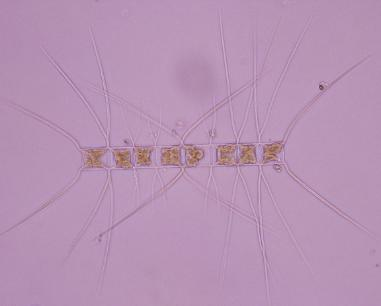
\includegraphics[height=3.6cm]{resize.jpg}
   \caption{}
  \end{subfigure}
  \begin{subfigure}{0.3\textwidth}
    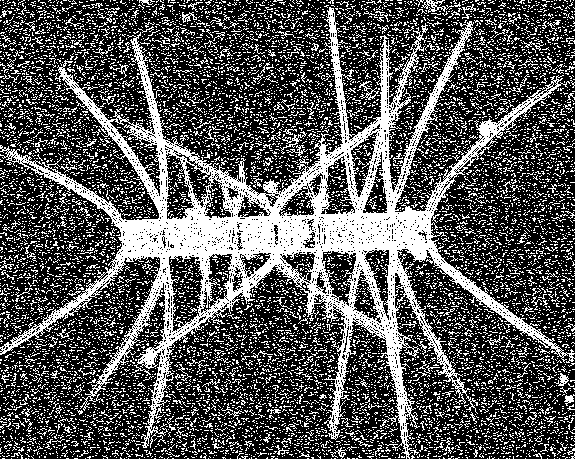
\includegraphics[height=3.6cm]{bingji1svm.png}
    \caption{}
  \end{subfigure}
  \begin{subfigure}{0.3\textwidth}
    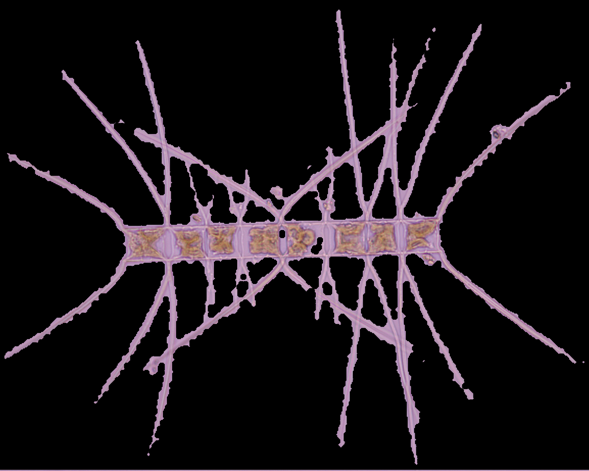
\includegraphics[height=3.6cm]{bingji1result.png}
    \caption{}
  \end{subfigure}
  \\
  \begin{subfigure}{0.3\textwidth}
    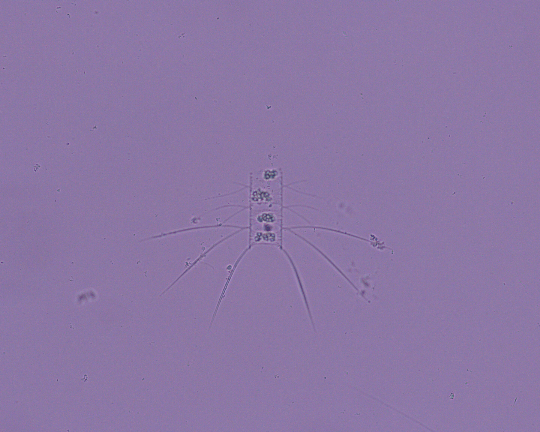
\includegraphics[height=3.6cm]{bingji2.png}
    \caption{}
  \end{subfigure}
 \begin{subfigure}{0.3\textwidth}
    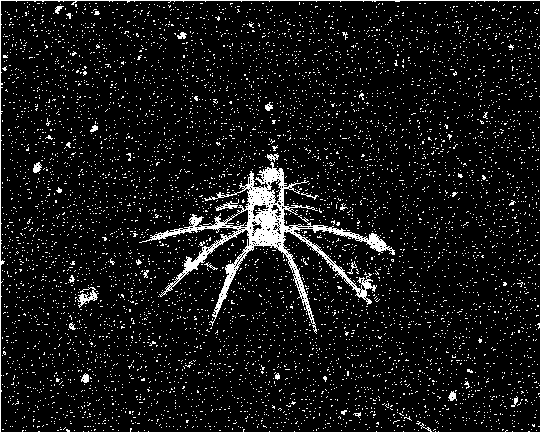
\includegraphics[height=3.6cm]{bingji2svm.png}
    \caption{}
  \end{subfigure}
 \begin{subfigure}{0.3\textwidth}
    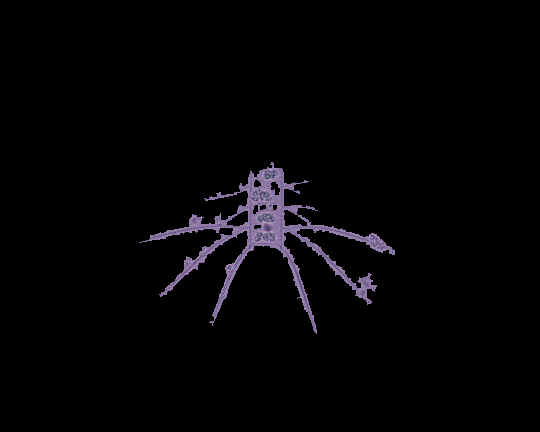
\includegraphics[height=3.6cm]{bingji2result.png}
    \caption{}
  \end{subfigure}
 \\
 \begin{subfigure}{0.3\textwidth}
    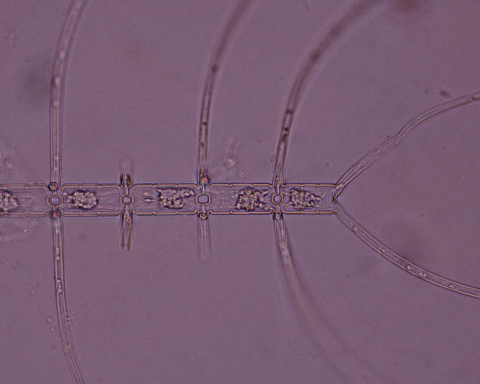
\includegraphics[height=3.6cm]{beifang.png}
    \caption{}
  \end{subfigure}
  \begin{subfigure}{0.3\textwidth}
    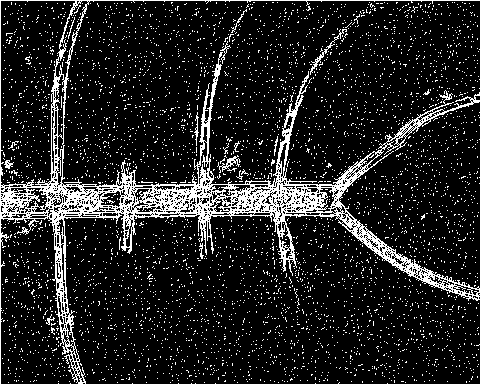
\includegraphics[height=3.6cm]{beifangsvm.png}
    \caption{}
  \end{subfigure}
   \begin{subfigure}{0.3\textwidth}
    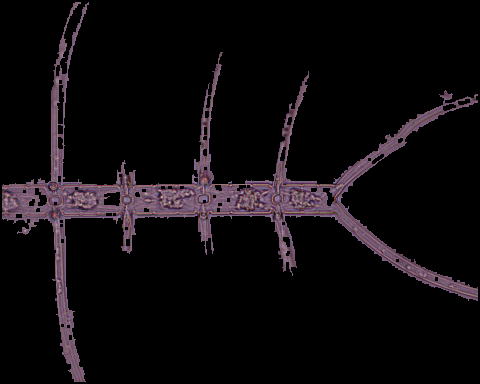
\includegraphics[height=3.6cm]{beifangresult.png}
    \caption{}
  \end{subfigure}
  \\
   \begin{subfigure}{0.3\textwidth}
    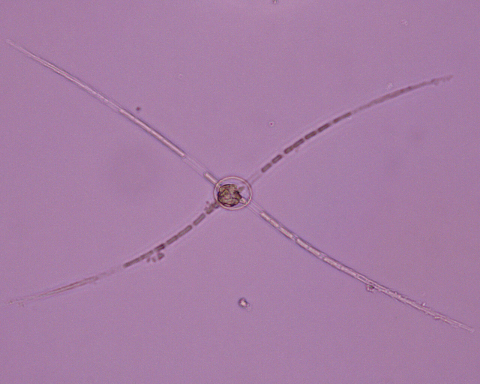
\includegraphics[height=3.6cm]{danmai.png}
    \caption{}
  \end{subfigure}
   \begin{subfigure}{0.3\textwidth}
    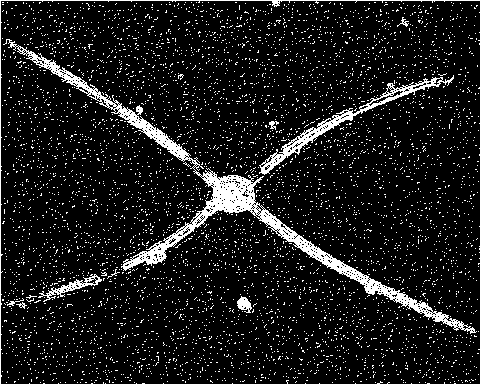
\includegraphics[height=3.6cm]{danmaisvm.png}
    \caption{}
  \end{subfigure}
   \begin{subfigure}{0.3\textwidth}
    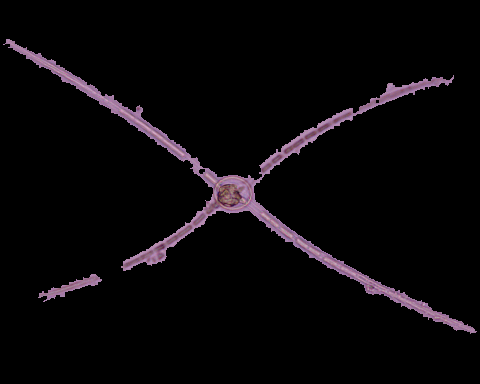
\includegraphics[height=3.6cm]{danmairesult.png}
    \caption{}
  \end{subfigure}
  \caption{支持向量机分类结果和最终分割结果。第一列为原始角毛藻显微图像,第二列为对应的支持向量机分类结果,第三列为采用形态学操作等后续处理过程产生的最终分割结果。}
  \label{svm}
\end{figure}


\section{本章小结}
本章将图像分割问题视为像素分类问题,采用支持向量机对原始图像中的每个像素进行分类。本章详细介绍了支持向量机算法的理论知识和实现过程,然后给出了实验的具体实施步骤以及最终分割结果。实验表明本文的分割方法能够获得较为理想的效果,最终的分割结果可以将图像中复杂的角毛部分较为精确和完整地提取出来。

 
